\subsection{Stability}
    \begin{minipage}{0.39\linewidth}
        \titel{system behaviour}
        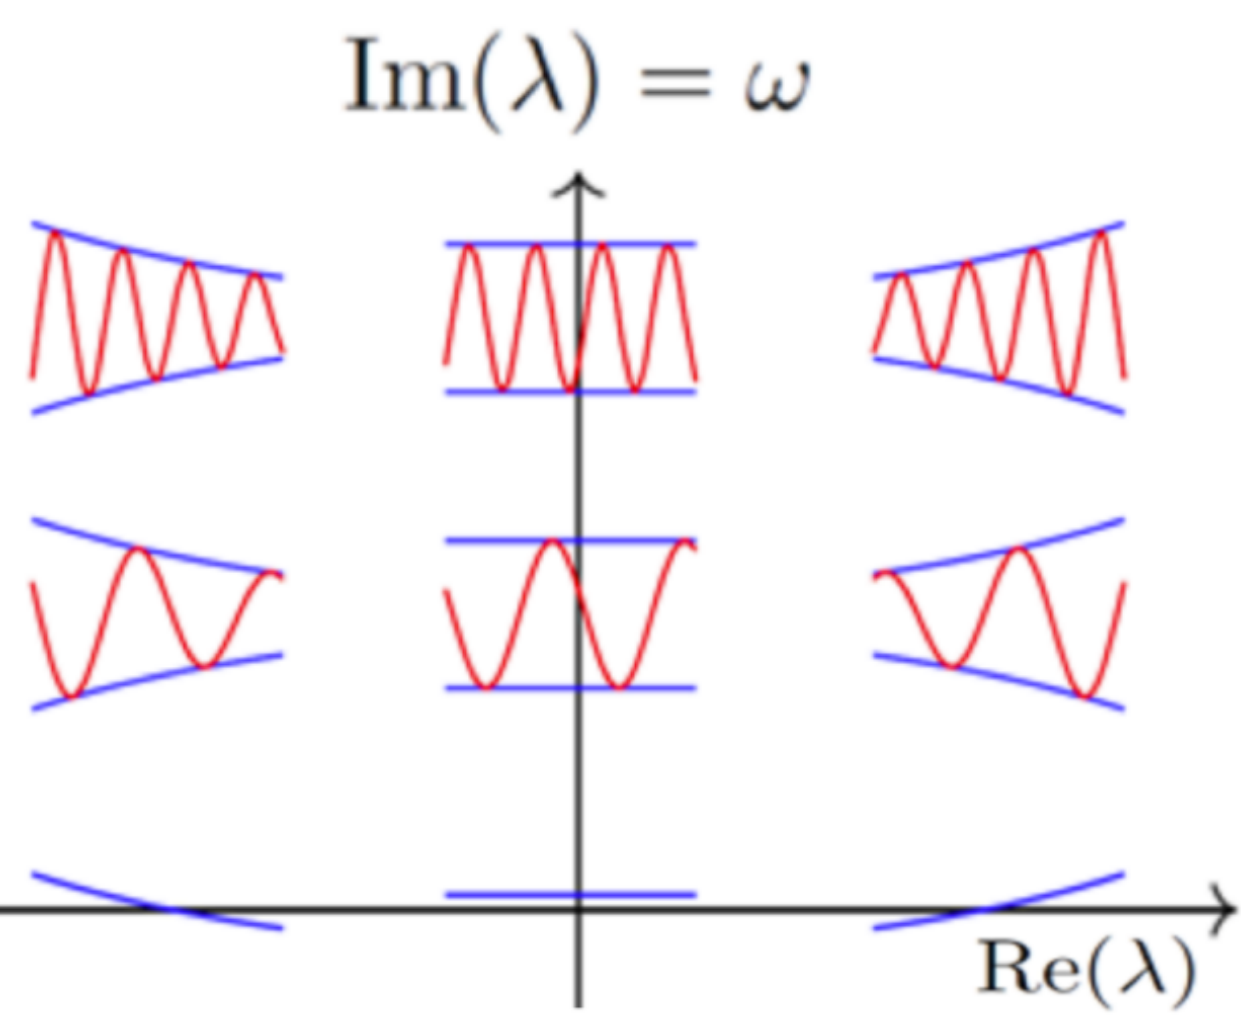
\includegraphics[width = \linewidth]{src/images/eigenvalue_response.png}
        $\lambda =$ eigenvalues of A
    \end{minipage}
    \begin{minipage}{0.59\linewidth}
        \titel{Lyapunov stable}
        \begin{align*}
            \lim_{t \rightarrow \infty} x(t) \neq \pm \infty \Leftrightarrow Re(\lambda_i) \leq 0\\
            \text{No repeated } \lambda_i \text{ with } Re(\lambda_i) = 0
        \end{align*}
%
        \titel{Asymptotically stable}
        \begin{align*}
            \lim_{t \rightarrow \infty} x(t) = 0 \Leftrightarrow Re(\lambda_i) < 0
        \end{align*}
%
        \titel{BIBO (Bounded Input Bounded Output)}
        \begin{align*}
            \lim_{t \rightarrow \infty} y(t) \neq \pm \infty, x_0 = 0
        \end{align*}
    \end{minipage}

    \begin{tabu}{|X[6] X X[3]|}
        \hline
        asymptotically stable & $\rightarrow$ & lyapunov stable\\
        asymptotically stable & $\rightarrow$ & BIBO stable\\
        ? & $\leftarrow$ & BIBO stable\\
        Lyap. stable or unstable & $\rightarrow$ & ?\\
        Lyap. stable or unstable & $\leftarrow$ & BIBO unstable\\
        \hline
    \end{tabu}

    \subsubsection{Unstable}
    $\lim_{t \rightarrow \infty} x(t) = \pm \infty \Leftrightarrow Re(\lambda_i) > 0 \text{for at least one i}$